% Introduction

% Problem:
% - Problem and analysis:
% - System diagram (what we want to build):
% Daniel has already made a nice diagram of this

% Robot control:
% Theory:
% - functionality
% - step/control sequence
% Implementation: (programming)
% - programming/framework etc.

% Map handling:
% Theory (how we did and thoughts):
% - Introduction (what is map handling about, what have we covered here, problems we want to solve)
% - Analysis of map input6
% - Converting analog map to digital map (intro)
% - 
% Implementation:
% - Read, compare, update 

% read google docs

% I can use \subsection and \subsubsection :)

\chapter{Map handling}
\label{ch:map} % chapter label
The rescue robot should be able follow a given path from start to finish, based on a predefined map.
A map provides useful information about whether areas of the map are accessible or not. This is an important element in path-finding. Map data can be given to the robot prior to its physical presences at a location. Once the robot is at the starting point, it has to rely on its sensors for updated information about the surroundings.

A structured way of storing the required map data for different maps was designed. 
The goal was to not only make it readable by the microcontroller, 
but also user-friendly enough to let a person design different maps for testing purposes of this project.

Existing pathfinding algorithms such as Diekstra and A* was studied, 
in order to understand what input data such algorithms typically would require. 
The pathfinding algorihtm implemented in this project is further described in chapter \ref{ch:path}. 
\newpage

\section{Map requirements}
\label{ch:map_requirements}
Maps come in many different shapes and sizes. 
These can sometimes prove to be hard for humans to interpret correctly, and possibly even harder for computers.
Two different examples of floor plans can be seen in figure \ref{fig:floor_plans}.

\begin{figure}[htp]
    \centering
    \caption{Examples of floor plans for different maps}
    \subfloat[Section of AAU Esbjerg]{%
        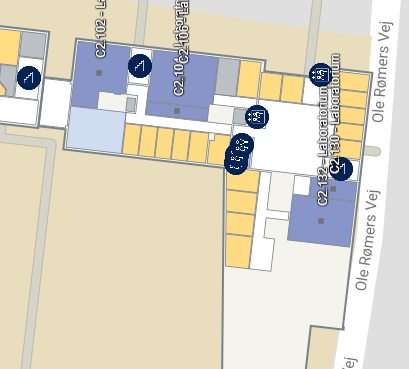
\includegraphics[width=0.48\textwidth]{figures/map/floorplan_aau.png}%
        }%
    \hfill%
    \subfloat[School layout example]{%
        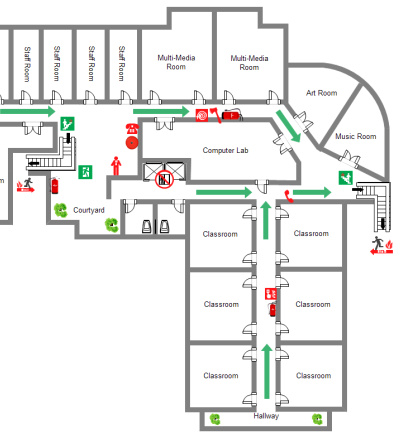
\includegraphics[width=0.48\textwidth]{figures/map/floorplan_school.png}%
        }%
    \label{fig:floor_plans}
\end{figure}
% https://www.edrawsoft.com/school-layout-example.php

Such maps are often very visual, providing a lot of detail and information to the human reader.
The way the information is structured differently, makes it very hard to be interpreted by a single program.

For this project it was decided that a simplified map would be sufficient.
A map must provide certain information that could easily be interpreted by the micro controller.

Table \ref{table:map_data} shows the chosen data the map should include, as well as some areas that has been delimited from. 
It is assessed that the delimited parts are interesting areas of extra considerations, 
but unnecessary in order to work with the basic principles of path-finding.

\begin{center}
	\begin{tabular}{|l|}
		\hline
		Data to be included \\ 
		\hline
		Map dimensions \\
		Start position \\
		Finish position \\
		Walls \\
		Objects (?) \\
		\hline
	\end{tabular}
	\begin{tabular}{|l|}
		\hline
		Data to delimit from \\ 
		\hline
		Differences in height (plans, stairs etc.) \\
		Door openings \\
		Ground surface (slipping, traction) \\
		Objects (?) \\
		Other (?) \\
		\hline
	\end{tabular}
	\captionof{table}{Map data}
	\label{table:map_data}
\end{center}


\section{Map coordinates}
\label{sec:map_coordinates} % section label

\begin{figure}[htp]
    \centering
    \caption{2D array}
    \subfloat[2D array]{%
        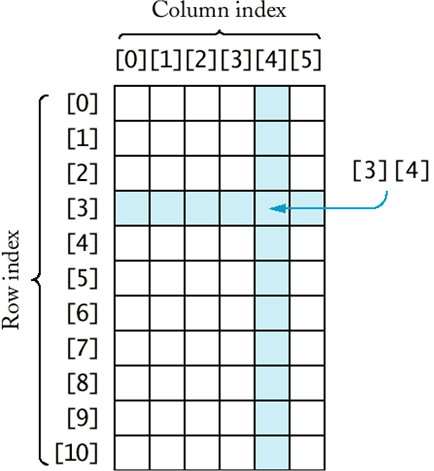
\includegraphics[width=0.5\textwidth]{figures/map/2d-array.png}%
        }%
    \label{fig:2d-array}
\end{figure}
%https://i.stack.imgur.com/tFdLk.gif

\section{Map design}
\label{sec:map_design} % section label
Show the map + wiki\\
Explain we made the map size dynamic to handle any map size
Explain how to store wall as hex value?\\
\\
\begin{figure}[htp]
    \centering
    \caption{5x5 map}
    \subfloat[5x5 map]{%
        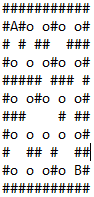
\includegraphics{figures/map/5x5map.png}%
        }%
    \label{fig:5x5map}
\end{figure}

\section{Check map}
\label{sec:map_check} % section label
Remember we have a chapter dedicated to scan.\linebreak
Based on scenario things might have dramatically changed, even to the point of map being useless. Explain how map is updated.

\section{Implementation}
\label{sec:map} % section label
Code here, or parts of code under each section?\\
\\
Like with many others,
is the first step in Dijkstra's algorithm to reduce the map to the necessary minimum.
After this reduction, the map only consists of \emph{nodes} and \emph{edges}.
An edge connects two nodes together and has one integer \emph{travel cost}.
In this integer is stored how much it costs to traverse along that edge,
measured in the metric that should get optimized (in our case distance).


